\begin{frame}{Results}
    \begin{itemize}
        \item The \mlblink algorithm is evaluated in isolation (no \mlblinkui)
        \item Compare the \mlblink algorithm to randomly searching for anomalies
            \begin{itemize}
                \item Recommend an item with probability of $1/5005 = 0.0002$
                \item In 200 time steps $7 \times 1/5005 \times 200 = 0.27$ anomalies
            \end{itemize}
        \item A total of 7 artificial anomalies were created
    \end{itemize}
\end{frame}

\begin{frame}{Results}
    \begin{table}[H]
        \centering
            \begin{tabular}{| c | c | c |}
                \hline
                  Image Key & \usno Band & \panstarrs Band \\
                \hline
                  13 & \texttt{blue1} & \texttt{g} \\
                \hline
                  13 & \texttt{blue2} & \texttt{g} \\
                \hline
                  56 & \texttt{blue1} & \texttt{g} \\
                \hline
                  56 & \texttt{blue2} & \texttt{g} \\
                \hline
                  679 & \texttt{ir} & \texttt{z} \\
                \hline
                  831 & \texttt{red1} & \texttt{r} \\
                \hline
                  831 & \texttt{red2} & \texttt{r} \\
                \hline
            \end{tabular}
        \caption{Complete list of anomalies that were created to evaluate the \mlblink algorithm.}
    \end{table}
\end{frame}

\begin{frame}{Results}
    \begin{figure}
      \centering
      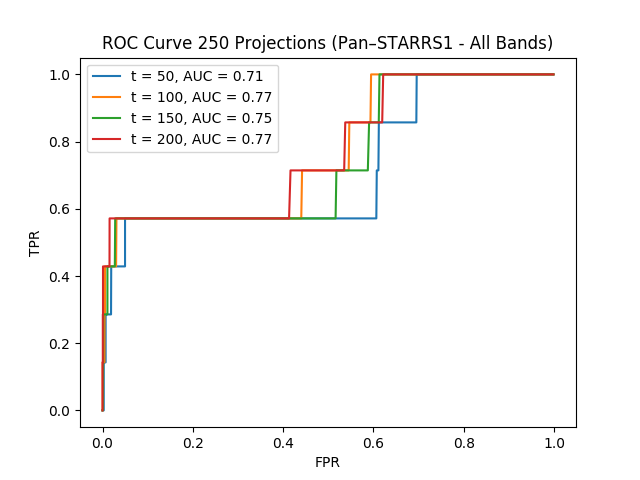
\includegraphics[
            width=0.7\textwidth,
            keepaspectratio
      ]{report/images/results/250_all_bands/250_all_bands_3_anomalies_t_200.png}
      \caption{ROC curve and AUC of the evaluation of the \mlblink algorithm using 250 projections for a total of 200 time steps.}
    \end{figure}
\end{frame}

\begin{frame}{Results}
    \begin{figure}
      \centering
      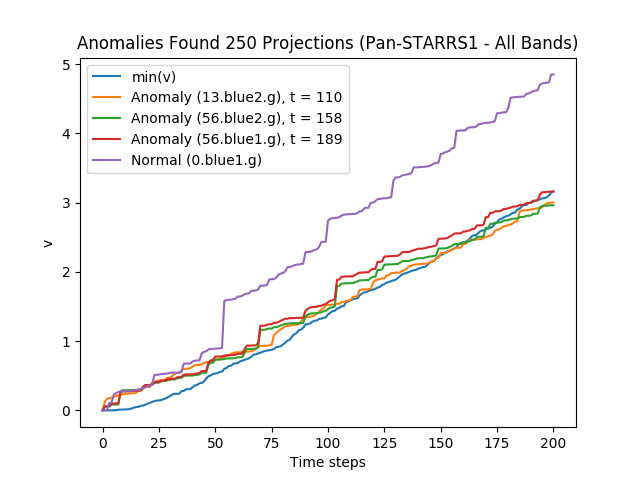
\includegraphics[
            width=0.7\textwidth,
            keepaspectratio
      ]{report/images/results/250_all_bands/found_250_all_bands_3_anomalies_t_200.png}
      \caption{Evaluation of known anomalies (that the \mlblink algorithm found) versus normal observations in comparison to the $\min(v)$ value at each time step.}
    \end{figure}
\end{frame}

\begin{frame}{Results}
    \begin{figure}
      \centering
      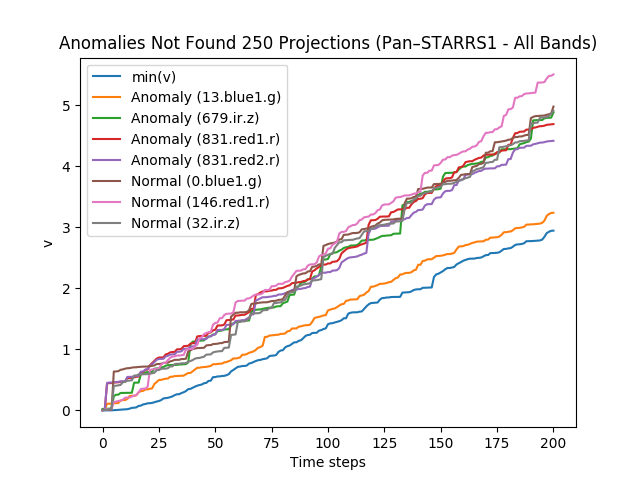
\includegraphics[
            width=0.7\textwidth,
            keepaspectratio
      ]{report/images/results/250_all_bands/not_found_250_all_bands_4_anomalies_t_200.png}
      \caption{Evaluation of known anomalies (that the \mlblink algorithm could not find) versus normal observations in comparison to the $\min(v)$ value at each time step.}
      \label{fig:evaluation:v-versus-t:not-found}
    \end{figure}
\end{frame}

% \begin{frame}{Results}
%     \begin{itemize}
%         \item All artificial anomalies evaluated close to the $\min(v)$ of any time step are in the \panstarrs color--band \texttt{g}
%         \item Next step is to evaluate each \panstarrs band in isolation
%     \end{itemize}
% \end{frame}

% \begin{frame}{Results}
%     \begin{table}[H]
%         \centering
%             \begin{tabular}{| c | c | c |}
%                 \hline
%                   Image Key & \usno Band & \panstarrs Band \\
%                 \hline
%                   13 & \texttt{blue1} & \texttt{g} \\
%                 \hline
%                   13 & \texttt{blue2} & \texttt{g} \\
%                 \hline
%                   56 & \texttt{blue1} & \texttt{g} \\
%                 \hline
%                   56 & \texttt{blue2} & \texttt{g} \\
%                 \hline
%                   679 & \texttt{ir} & \texttt{z} \\
%                 \hline
%                   831 & \texttt{red1} & \texttt{r} \\
%                 \hline
%                   831 & \texttt{red2} & \texttt{r} \\
%                 \hline
%             \end{tabular}
%         \caption{Complete list of anomalies that were created to evaluate the \mlblink algorithm.}
%     \end{table}
% \end{frame}

% \begin{frame}{Results}
%     \begin{figure}[H]
%         \centering
%         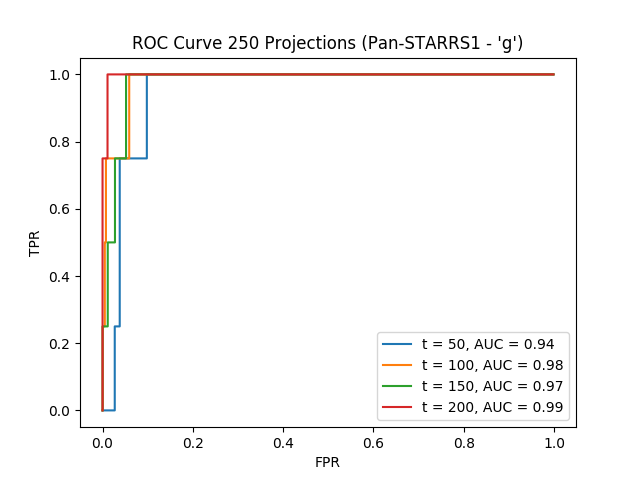
\includegraphics[
%             width=0.7\textwidth,
%             keepaspectratio
%         ]{report/images/results/250_panstarr_g/250_panstarr_g_3_anomalies_t_200.png}
%         \caption{ROC curve and AUC achieved by the \mlblink algorithm when evaluating observations in the \panstarrs color--band \texttt{g} only (versus \usno color--bands \texttt{blue1} and \texttt{blue2}) using 250 projections for dimensionality reduction.}
%     \end{figure}
% \end{frame}

% \begin{frame}{Results}
%     \begin{figure}[H]
%         \centering
%         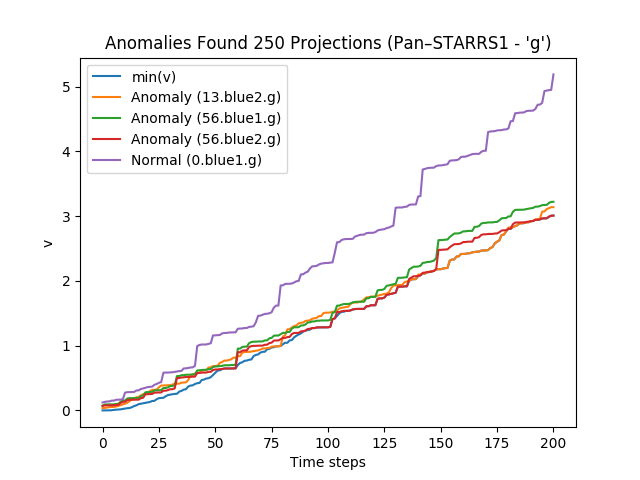
\includegraphics[
%             width=0.7\textwidth,
%             keepaspectratio
%         ]{report/images/results/250_panstarr_g/found_250_panstarr_g_3_anomalies_t_200.png}
%         \caption{Evaluation of known anomalies that were found by the \mlblink algorithm when evaluating the \panstarrs color--band \texttt{g} (versus \usno color--bands \texttt{blue1} and \texttt{blue2}) in isolation using 250 projections for dimensionality reduction.}
%     \end{figure}
% \end{frame}

% \begin{frame}{Results}
%     \begin{figure}[H]
%         \centering
%         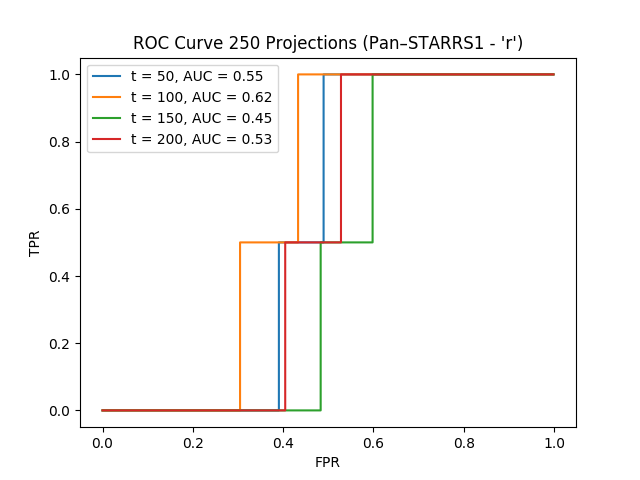
\includegraphics[
%             width=0.7\textwidth,
%             keepaspectratio
%         ]{report/images/results/250_panstarr_r/250_panstarr_r_0_anomalies_t_200.png}
%         \caption{ROC curve and AUC achieved by the \mlblink algorithm when evaluating observations in the \panstarrs color--band \texttt{r} only (versus \usno color--bands \texttt{red1} and \texttt{red2}) using 250 projections for dimensionality reduction.}
%     \end{figure}
% \end{frame}

% \begin{frame}{Results}
%     \begin{figure}[H]
%         \centering
%         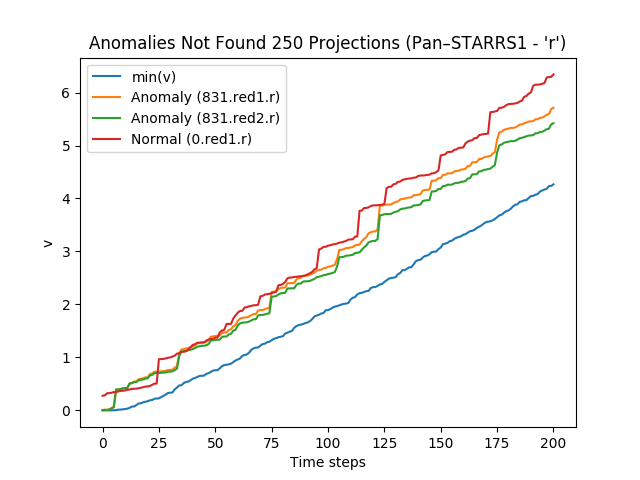
\includegraphics[
%             width=0.7\textwidth,
%             keepaspectratio
%         ]{report/images/results/250_panstarr_r/not_found_250_panstarr_r_2_anomalies_t_200.png}
%         \caption{Evaluation of known anomalies that were not found by the \mlblink algorithm when evaluating the \panstarrs color--band \texttt{r} (versus \usno color--bands \texttt{red1} and \texttt{red2}) in isolation using 250 projections for dimensionality reduction.}
%     \end{figure}
% \end{frame}

% \begin{frame}{Results}
%     \begin{figure}[H]
%         \centering
%         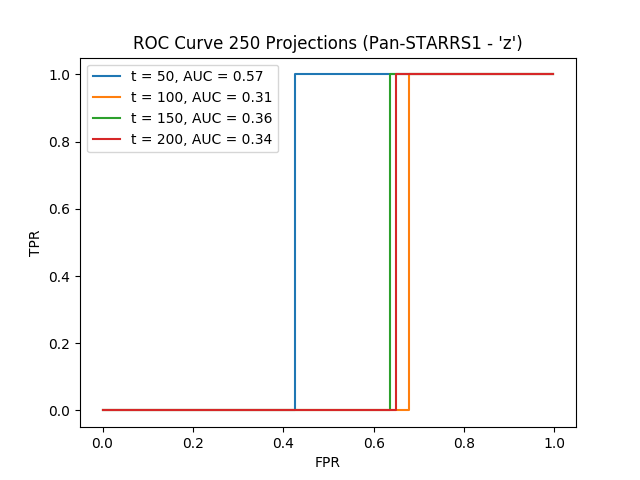
\includegraphics[
%             width=0.7\textwidth,
%             keepaspectratio
%         ]{report/images/results/250_panstarr_z/250_panstarr_z_0_anomalies_t_200.png}
%         \caption{ROC curve and AUC achieved by the \mlblink algorithm when evaluating observations in the \panstarrs color--band \texttt{z} only (versus \usno color--band \texttt{ir}) using 250 projections for dimensionality reduction.}
%         \label{fig:evaluation:roc:panstarrs:z}
%     \end{figure}
% \end{frame}

% \begin{frame}{Results}
%     \begin{figure}[H]
%         \centering
%         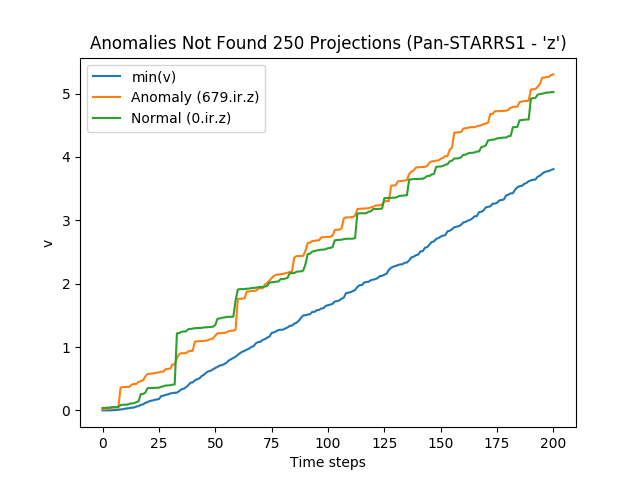
\includegraphics[
%             width=0.7\textwidth,
%             keepaspectratio
%         ]{report/images/results/250_panstarr_z/not_found_250_panstarr_z_1_anomalies_t_200.png}
%         \caption{Evaluation of known anomalies that were not found by the \mlblink algorithm when evaluating the \panstarrs color--band \texttt{z} (versus \usno color--bands \texttt{ir}) in isolation using 250 projections for dimensionality reduction.}
%     \end{figure}
% \end{frame}

%%%%%% Average Pooling %%%%%%
% \begin{frame}{Results}
%     \begin{itemize}
%         \item Same experiments were conducted using average pooling with a kernel of size $7 \times 7$ for dimensionality reduction
%         \item Results when using average pooling were unstable and difficult to reproduce
%         \item It was decided to not continue these experiments further due to their instability and lack of reproducibility
%     \end{itemize}
% \end{frame}

% \begin{frame}{Results}
%     \begin{figure}[H]
%         \centering
%         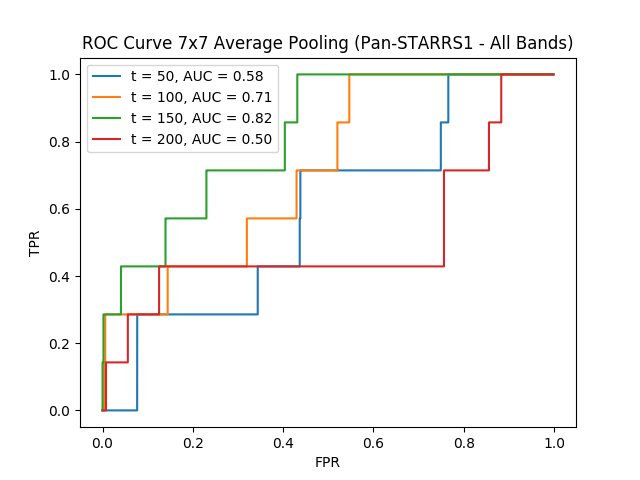
\includegraphics[
%             width=0.7\textwidth,
%             keepaspectratio
%         ]{report/images/results/7x7_all_bands_4/7x7_all_bands_2_anomalies_t_200.png}
%         \caption{ROC curve and AUC when using average pooling with a kernel of size $7 \times 7$ for a total of 200 time steps}
%     \end{figure}
% \end{frame}

% \begin{frame}{Results}
%     \begin{figure}[H]
%         \centering
%         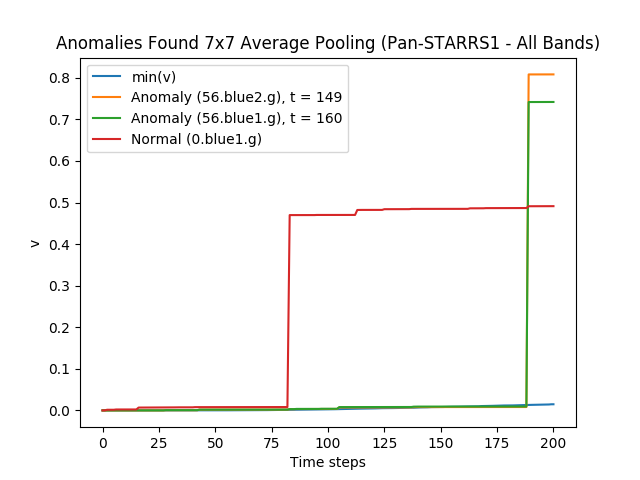
\includegraphics[
%             width=0.7\textwidth,
%             keepaspectratio
%         ]{report/images/results/7x7_all_bands_4/found_7x7_all_bands_2_anomalies_t_200.png}
%         \caption{Evaluation of the $v$ value of known anomalies and a normal observation as the \mlblink algorithm is taught over time when using average pooling for dimensionality reduction}
%     \end{figure}
% \end{frame}